\section{Verification of long ping times}
\label{sec:verification}

In this section, we address doubts that long observed ping
times are real: that they are a product of ISI's probing scheme, that
they might be caused by errors in a particular data set, or that they might derive from
discrimination against ICMP.

\subsection{Are high latencies observed by other probing schemes?}

Some of the latencies in Table~\ref{tbl:grand_2015} are so high that
we considered if they could be artifacts of ISI's probing scheme. We
investigate latencies obtained using two other probing techniques,
Zmap and scamper, and check if the high latencies observed in the ISI datasets are reproducible.
%  We confirm that each observes the
% occurrence of long ping times.
% We use the scamper tool to probe a subset of high
% latency addresses and 



\subsubsection*{Does Zmap observe high latencies?}
% \paragraph{Zmap observes high latencies}

We check for high latencies using the Zmap scanner~\cite{durumeric2013zmap}. 
%
As part of our extension of the ICMP probing module in the
Zmap scanner, we also embed the probe send time into the echo request,
and extract it from the
echo response, allowing us to estimate the RTT, albeit without the
precision of kernel send timestamps.
%
% Zmap collected the data and made
% it available for download at \url{scans.io}.

Zmap has performed these scans since April 2015. Scans have been conducted over a range of different times,
different days of the week and across four months in 2015 (as of Sep
5, 2015), as shown in Table~\ref{tbl:scans}. Typically, scans were performed on Sundays or Thursdays, beginning
at noon UTC time. However, the scans on April 17, May 22, and June 15
were conducted on other days and at other times, increasing diversity. Each Zmap scan
takes 10 and a half hours to complete and recovers Echo Responses from
around 350M addresses.
%

\begin{table}[tb]
  \begin{center}
    \begin{small}
  \begin{tabular}{r|c|c|c}
    \hdr{Scan Date} & \hdr{Day} & \hdr{Begin Time} & \hdr{Echo Responses} \\
    \hline
    \textbf{Apr 17, 2015} & Fri & 02:44 & 339M\Tstrut \\
    \textbf{Apr 19, 2015} & Sun & 12:07 & 340M \\
    \textbf{Apr 23, 2015} & Thu & 12:07 & 343M \\
    \textbf{Apr 26, 2015} & Sun & 12:07 & 343M \\
    \textbf{Apr 30, 2015} & Thu & 12:08 &  344M \\
    \textbf{May 3, 2015} & Sun & 12:08 & 344M \\
    \textbf{May 17, 2015} & Sun & 12:09 &  347M \\
    \textbf{May 22, 2015} & Fri & 00:57 & 371M \\
    \textbf{May 24, 2015} & Sun & 12:09 &  369M \\
    \textbf{May 31, 2015} & Sun & 12:09 & 362M \\
    \textbf{Jun 4, 2015} & Thu & 12:10 & 368M \\
    \textbf{Jun 15, 2015} & Mon & 13:53 & 357M \\
    % \hline
    \textbf{Jun 21, 2015} & Sun & 12:11 & 368M \\
    % \hline
    \textbf{Jul 2, 2015} & Thu & 12:00 & 369M \\
    \textbf{Jul 5, 2015} & Sun & 12:00 & 368M \\
    \textbf{Jul 9, 2015} & Thu & 12:00 & 369M \\
    \textbf{Jul 12, 2015} & Sun & 12:00 & 367M \\
    \end{tabular}
    \end{small}
  \end{center}
    \caption{Zmap scan details: For each Zmap scan in
      Figure~\ref{fig:grand_zmap}, the table shows the date, day of the
      week, the time at which the scan began (in UTC time), and the number of
      destinations that responded with Echo Responses.}

\label{tbl:scans}
\end{table}

We choose all
available scans and 
analyze the distribution of
RTTs for the Echo Responses in
Figure~\ref{fig:grand_zmap}. 
%
Most responses arrive with low latency, having a median latency lower than
250ms for each scan.
%
However, ~5\% of addresses responded with RTTs greater than 1 second
in each scan. Further, 0.1\% of addresses responded with latencies exceeding
75 seconds in each scan although the 99.9th percentile
latency exhibited some variation: the May 22 scan had the lowest 99.9th percentile
latency (77 seconds) whereas the July 9 scan had the highest (102 seconds).
%
We infer from these nearly identical latency distributions that high latencies are persistent for a consistent fraction of addresses.
% To compare the distribution of RTTs requires choosing a
% comparable sample from the survey data, given that it
% reprobes addresses for weeks.  We used the latency of the
% first received ping from each address in the IT63c
% (20150206) and IT63w (20150117) datasets.  

% Figure~\ref{fig:zmap_vs_isi_2015} shows the distribution of RTTs. 5\%
% of addresses have latencies $>$ 1s in each.

% \begin{figure}[tbh]
% \centering
% \includegraphics[width=3in]{figs/zmap_vs_isi_2015}
% \caption{\label{fig:zmap_vs_isi_2015}%
% Distribution of RTTs for three Zmap scans and
% two ISI surveys performed in 2015. 5\% of addresses have latencies $>$
% 1s in each.
% }
% \end{figure}

\begin{figure}[tb]
% \centering
\begin{center}
\includegraphics[width=3in]{timeouts/figs/grand_zmap}
\end{center}
\caption{\label{fig:grand_zmap}%
Distribution of RTTs for all Zmap scans performed in 2015. Around 5\%
of addresses have latencies greater than 1s in each scan, and 0.1\% of addresses observed latencies in excess of 75s.
}
\end{figure}

% \vspace{-0.1in}

\subsubsection*{Does scamper also observe high latencies?}
% \paragraph{Scamper also observes high latencies}
Both ISI and Zmap probe millions of addresses, and we investigate
whether latencies are affected by these probing schemes
triggering rate-limits or firewalls. We select a small sample of
addresses that are likely to have high latencies from the
ISI dataset, probe them using scamper~\cite{luckie2010scamper}, and check for unusually high latencies.

In the 2011 - 2013
ISI dataset, 20,095 IP
addresses had at least 5\% of their pings with latencies 100 seconds and above. We chose 2000 random IP addresses from
this subset and sent 1000 pings to them, once every 10 seconds using
scamper~\cite{luckie2010scamper} and analyzed the responses. 
In this
analysis, we used scamper's default packet response matching
mechanism: so long as scamper continues to run, received responses
will be matched with sent packets. Because we used scamper's defaults,
scamper ceased to run 2 seconds after the last packet was sent, so
we missed responses to the last few pings that arrived after
scamper ceased running. Although scamper can
be configured to wait longer for responses, in later analyses, we ran tcpdump simultaneously and matched
responses to sent packets separately.

Of the 2000 addresses, 1244 responded to our probes.
Figure~\ref{fig:cdf_high_rtt_ips} shows the percentile latency per IP
address. The 95th percentile latency for 50\% of the addresses is now
considerably lower, at 7.3s. This suggests that addresses prone to extremely high
latencies vary with time: we investigate addresses with
this behavior further in Section~\ref{sec:causes}. 

Nevertheless, Figure~\ref{fig:cdf_high_rtt_ips} shows that scamper
also observes some instances of very high latencies. 17\%
of addresses observe latencies greater than 100 seconds for 1\%
of their pings. We therefore rule out the possibility that the high
latencies are a product of the probing scheme.

% , and show that they addresses tend
% to be from cellular Autonomous Systems which exhib


\begin{figure}[tb]
\begin{center}
% \centering
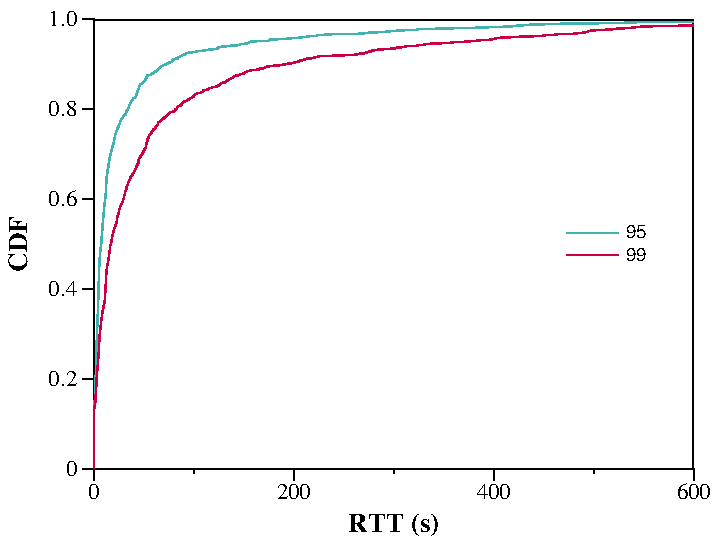
\includegraphics[width=3in]{timeouts/figs/cdf_high_rtt_guys_grand}
\end{center}
\caption{\label{fig:cdf_high_rtt_ips}%
Confirmation of high latency: Percentile latency per IP address for
2000 randomly chosen IP addresses from ISI's 2011 - 2013 surveys that had $>$ 5\% of pings with
latencies 100s and above. Each point represents an IP address and the
lines represent the percentile latency from that IP address. 17\% of
them continue to observe 1\% of their pings with
latencies $>$ 100s.
}
\end{figure}

% \subsection{Are ISI's sampled addresses representative?}

% ISI's methodology involves probing a sample of the address
% space.  It would be reasonable to expect that perhaps this
% sampling affects observed latencies.  An underestimate might
% occur because a fraction of the ISI survey prefixes have
% been repeated since 2006, so such addresses may be in a more
% established part of the network.  On the other hand,
% latencies might be overestimated by bad luck, repeatedly probing a
% particularly slow prefix. 


% 0.1% of pings arrived after: April : 90, May : 77,  June : 83, Julys
% : 102

% per dataset analysis (time)
\ninput{timeouts/per_dataset}

\ninput{timeouts/is_it_icmp}

\subsection{Summary}

In this section, we confirmed that extremely high latencies are also observed by
techniques besides ISI's. We find that the high latencies are
not a result of a few individual ISI datasets, even though some
did appear atypical.  Further, high latencies affect all
protocols the same. 

We also found that the prevalence of high latencies has been increasing
since 2011. In 2015, a consistent 5\% of addresses have
latencies greater than a second. 
